% Chương 2: Cơ sở lý thuyết và các nghiên cứu liên quan (bản rút gọn)
\chapter{CƠ SỞ LÝ THUYẾT VÀ CÁC NGHIÊN CỨU LIÊN QUAN}
\label{chap:co-so}

Chương này đi từ bài toán tới công cụ, rồi từ công cụ tới giới hạn của chúng. Mục \ref{sec:thuoc-tinh} xác định những thuộc tính làm cho một văn bằng số đáng tin. Mục \ref{sec:ssi} và \ref{sec:ha-tang} trình bày mô hình định danh tự chủ cùng các khối kỹ thuật hiện thực hoá nó; Mục \ref{sec:mat-ma} trình bày nền tảng mật mã. Mục \ref{sec:blockchain} xem xét vai trò của blockchain theo hướng phản biện. Hai mục cuối dùng lăng kính ba tầng niềm tin để khảo sát các hệ thống hiện có và phân loại khoảng trống nghiên cứu.

\section{Văn bằng số và các thuộc tính của sự tin cậy}
\label{sec:thuoc-tinh}

Có thể phân biệt ba thế hệ biểu diễn văn bằng. Văn bằng giấy dựa vào đặc trưng khó sao chép của vật thể và vào sổ gốc ở nơi cấp. Văn bằng số hoá (tệp PDF, ảnh quét, bản ghi trên cổng tra cứu) cải thiện việc lưu trữ và phân phối nhưng giữ nguyên cơ chế niềm tin: một tệp PDF sửa được, còn bản ghi trên cổng chỉ đáng tin bằng tổ chức vận hành cổng. Thế hệ thứ ba mới thực sự thay đổi kiến trúc: thông tin đủ để kiểm chứng được nhúng vào chính văn bằng, gồm chữ ký số trên toàn bộ nội dung, tham chiếu tới nơi tra khoá công khai của bên ký và tham chiếu tới nơi tra trạng thái hiệu lực. Bên xác minh làm phép kiểm tra trên dữ liệu mình đang giữ. Tổ chức không biến mất khỏi bức tranh, nhưng chỉ tham gia một lần lúc phát hành và trong việc duy trì trạng thái, thay vì tham gia vào từng lần xác minh.

Tổng hợp từ mô hình dữ liệu của W3C \cite{W3C_VCDM2025} và các tài liệu nền về định danh tự chủ \cite{Preukschat2021, Sedlmeir2021}, một văn bằng số đáng tin cần đồng thời ba thuộc tính độc lập:

\begin{itemize}
    \item \textbf{Xác thực nguồn gốc}: văn bằng chứng minh được nó do một thực thể xác định phát hành, kiểm chứng được mà không cần liên hệ thực thể đó.
    \item \textbf{Toàn vẹn nội dung}: mọi thay đổi sau khi phát hành, dù chỉ một ký tự, đều bị phát hiện.
    \item \textbf{Trạng thái hiệu lực theo thời gian}: văn bằng phản ánh đúng trạng thái tại thời điểm xác minh, kể cả khi đã bị thu hồi, tạm đình chỉ hay hết hạn.
\end{itemize}

Ba thuộc tính này không thay thế được cho nhau. Chữ ký số bảo đảm hai thuộc tính đầu \emph{tại thời điểm ký}, nhưng một văn bằng đã bị thu hồi vì gian lận vẫn mang chữ ký hợp lệ về mặt toán học. Ngược lại, một hệ thống chỉ theo dõi trạng thái không phát hiện được nội dung bị sửa sau khi cấp, vì trạng thái bản ghi vẫn là ``đang hiệu lực''. Mục \ref{sec:xac-minh} và thí nghiệm ở Mục \ref{sec:dg-chuc-nang} cho thấy lỗ hổng này có thật. Ngoài ba thuộc tính trên còn một thuộc tính thứ tư quyết định giá trị thực tế của văn bằng là \emph{thẩm quyền của bên phát hành}, thuộc một tầng khác và được phân tích ở Mục \ref{sec:ba-tang}.

\section{Định danh tự chủ}
\label{sec:ssi}

\subsection{Từ định danh tập trung đến định danh tự chủ}

Theo NIST, danh tính số là biểu diễn dạng số của một tập thuộc tính về một chủ thể trong giao dịch điện tử \cite{NIST_SP800_63_3}; còn định danh là chuỗi ký tự phân biệt duy nhất một thực thể trong một hệ thống. Một thực thể có thể có nhiều định danh trên nhiều hệ thống, và đó chính là nguồn gốc của tình trạng phân mảnh. Mühle và cộng sự mô tả quá trình tiến hoá của các mô hình quản lý định danh \cite{Muhle2018}: mô hình tập trung (mỗi tổ chức một hệ thống tài khoản), mô hình liên kết (nhiều dịch vụ dùng chung một nhà cung cấp định danh) và mô hình hướng người dùng (người dùng quyết định thuộc tính nào được chia sẻ). Dù khác nhau về mức phân tán, cả ba đều có chung một điểm: sự tồn tại của định danh phụ thuộc vào một tổ chức trung gian. Với văn bằng, loại dữ liệu cần giữ giá trị qua nhiều thập kỷ, đây là hạn chế nền tảng.

Định danh tự chủ (Self-Sovereign Identity, SSI) được Christopher Allen đề xuất năm 2016 như một phản hồi trực tiếp \cite{Allen2016}. Điểm khác biệt cốt lõi là tách \emph{quyền khẳng định thuộc tính} khỏi \emph{quyền kiểm soát dữ liệu}: trường đại học vẫn là bên duy nhất có thẩm quyền khẳng định một người đã tốt nghiệp, nhưng người học là bên giữ lời khẳng định đó và quyết định chia sẻ cho ai. Trong mười nguyên tắc Allen nêu ra, năm nguyên tắc liên quan trực tiếp tới văn bằng:

\begin{itemize}
    \item \textbf{Kiểm soát}: chủ thể là bên duy nhất tạo lập, cập nhật và vô hiệu hoá định danh của mình.
    \item \textbf{Đồng thuận}: mọi lần chia sẻ thông tin đều cần chủ thể đồng ý, cả về việc chia sẻ với ai lẫn chia sẻ gì.
    \item \textbf{Tính di động}: định danh và dữ liệu đi kèm dùng được trên nhiều hệ thống, không bị khoá vào một nền tảng.
    \item \textbf{Bảo vệ}: khi quyền của chủ thể xung đột với lợi ích của tổ chức, quyền của chủ thể được ưu tiên.
    \item \textbf{Tiết lộ tối thiểu}: chủ thể chỉ tiết lộ đúng lượng thông tin cần cho mục đích cụ thể.
\end{itemize}

Windley nhận xét rằng danh tính không phải một thực thể cố định mà là tập thuộc tính phù hợp với từng ngữ cảnh \cite{Windley2023}; một sinh viên liên thông giữa hai trường không cần một ``danh tính toàn diện'' mà chỉ cần trình bày đúng tập thuộc tính ngữ cảnh đó đòi hỏi. Các nguyên tắc trên mang tính định hướng và có lúc xung đột nhau, chẳng hạn nguyên tắc kiểm soát mâu thuẫn với nhu cầu khôi phục tài khoản: một hệ thống cho phép khôi phục khi mất khoá thì tất yếu phải có một bên khác tác động được lên định danh. Các khảo sát ghi nhận chưa triển khai nào thoả mãn đủ mười nguyên tắc cùng lúc \cite{Schardong2022, Muhle2018}.

SSI vận hành theo mô hình ba bên \cite{Preukschat2021}. \emph{Bên phát hành} (issuer) tạo và ký chứng thực; \emph{chủ thể} (holder) nhận, lưu giữ và quyết định trình bày; \emph{bên xác minh} (verifier) kiểm tra chứng thực mà không cần quan hệ trước với bên phát hành. Đặc điểm kiến trúc then chốt là dữ liệu và niềm tin đi theo hai đường khác nhau. Dữ liệu đi từ bên phát hành tới chủ thể rồi tới bên xác minh, hoàn toàn trong tay chủ thể. Niềm tin thì không đi theo đường đó: bên xác minh tự thiết lập niềm tin bằng cách tra hạ tầng công bố, nên chủ thể không làm sai lệch được kết quả xác minh dù nắm toàn bộ dữ liệu.

\subsection{Những gì SSI giải quyết và những gì còn bỏ ngỏ}

SSI đáp ứng trực tiếp hai trong ba vấn đề ở Mục \ref{sec:bai-toan}. Vì bằng chứng nằm trong chứng thực và khoá công khai được công bố độc lập, bên xác minh tự kiểm tra được kể cả khi dịch vụ của trường đã ngừng hoạt động. Vì định danh phi tập trung không thuộc về hệ thống nào, người học tích luỹ được chứng thực từ nhiều trường vào cùng một ví. Đồng thời mô hình này phù hợp tự nhiên với yêu cầu kiểm soát dữ liệu cá nhân \cite{LuatBVDLCN2025}, vì không cần gom hồ sơ học tập về một chỗ để phục vụ xác minh.

Còn hai giới hạn. Giới hạn thứ nhất là gánh nặng quản lý khoá: mất thiết bị hoặc mất cụm từ khôi phục có thể đồng nghĩa với mất toàn bộ định danh, và không tồn tại cơ chế ``quên mật khẩu'', vì chính sự tồn tại của cơ chế đó hàm ý có một bên khác kiểm soát được định danh. Nhiều triển khai chọn ví lưu ký để khắc phục, nhưng như vậy lại tái lập sự phụ thuộc vào bên thứ ba. Giới hạn thứ hai quan trọng hơn với đề tài: SSI không giải quyết bài toán thẩm quyền. Nó cho phép khẳng định ``chứng thực này do chủ khoá $K$ ký và chưa bị sửa'', nhưng không cho phép khẳng định ``chủ khoá $K$ có thẩm quyền cấp loại văn bằng này''. Trong một hệ sinh thái mở, ai cũng có thể sinh khoá và phát hành một chứng thực ``tốt nghiệp ngành Khoa học máy tính'' qua được mọi phép kiểm tra mật mã. SSI hiện thực hoá đầy đủ niềm tin ở tầng kỹ thuật nhưng để trống tầng thể chế.

\section{Hạ tầng kỹ thuật: DID, VC và ví định danh số}
\label{sec:ha-tang}

\subsection{Định danh phi tập trung}

DID là một URI dạng \texttt{did:<phương-thức>:<định-danh-riêng>} do W3C chuẩn hoá \cite{W3C_DIDCore2022}; phiên bản 1.1 đang ở trạng thái Candidate Recommendation \cite{W3C_DID11_2026}. Quyền kiểm soát DID thuộc về người giữ khoá tương ứng, nên bên thứ ba không thu hồi hay thay đổi được nó nếu không có khoá. Mỗi DID gắn với một DID Document chứa khoá công khai và các phương thức xác thực; trong đó trường \texttt{assertionMethod} chỉ định khoá nào được ký chứng thực, tách khỏi \texttt{authentication} để một khoá dùng cho đăng nhập và một khoá khác dùng cho cấp phát. Quá trình chuyển từ DID sang DID Document gọi là phân giải \cite{W3C_DIDResolution} và phụ thuộc vào phương thức.

\begin{table}[H]
\centering
\caption{So sánh các phương thức DID theo các tiêu chí liên quan tới văn bằng}
\label{tab:v2-did-method}
\renewcommand{\arraystretch}{1.25}
\small
\begin{tabular}{|p{2.0cm}|p{2.7cm}|p{2.2cm}|p{1.6cm}|p{4.6cm}|}
\hline
\textbf{Phương thức} & \textbf{Hạ tầng phân giải} & \textbf{Tính bất biến} & \textbf{Xoay khoá} & \textbf{Hệ quả với văn bằng} \\ \hline
\texttt{did:web} & DNS và HTTPS & Thấp & Có & Chủ tên miền sửa được lịch sử khoá, không đủ làm điểm neo thẩm quyền \\ \hline
\texttt{did:key} & Suy từ khoá công khai & Tuyệt đối & Không & Lộ khoá thì không thu hồi được; chỉ hợp với định danh tạm \\ \hline
\texttt{did:ethr} & Ethereum & Cao & Có & Bất biến tốt, chi phí biến động theo thị trường \\ \hline
\texttt{did:ion} & Bitcoin, Sidetree, IPFS & Rất cao & Có & Rẻ nhờ gộp lô nhưng độ trễ cao, phụ thuộc hạ tầng ngoài \\ \hline
\texttt{did:vnu} (đề xuất) & Hợp đồng Move và IPFS & Cao & Có, kèm phiên bản & Định danh và thẩm quyền chung một miền quản trị; bên xác minh cần bộ phân giải riêng \\ \hline
\end{tabular}
\end{table}

Bảng \ref{tab:v2-did-method} cho thấy mỗi phương thức sẵn có đều vướng một điểm. \texttt{did:web} \cite{DIDWeb2023} để chủ tên miền sửa được DID Document, kể cả sửa hồi tố. \texttt{did:key} \cite{DIDKey2022} không cho xoay khoá. \texttt{did:ethr} \cite{DIDEthr2023} và \texttt{did:ion} \cite{DIDION2021} phụ thuộc vào hệ sinh thái bên ngoài với chi phí và độ trễ không kiểm soát được. Cần lưu ý rằng khả năng truy xuất phiên bản cũ của DID Document \emph{không} phải lý do để thiết kế phương thức riêng: đặc tả phân giải đã có tham số \texttt{versionId} và \texttt{versionTime} \cite{W3C_DIDResolution}. Lý do thật gồm ba điểm, và cả ba là đánh đổi: sổ định danh và sổ thẩm quyền nằm trong cùng một miền để một lần truy vấn trả lời cả ``khoá nào'' lẫn ``có quyền gì''; cơ quan quản trị kiểm soát được chi phí; và chủ thể dùng một cặp khoá cho cả ký chứng thực lẫn ký giao dịch. Cái giá là phương thức chưa đăng ký với W3C nên khả năng liên thông giảm.

\subsection{Chứng thực, bản trình bày và trạng thái}

Một VC gồm siêu dữ liệu (định danh, loại, bên phát hành, thời điểm phát hành và hết hạn), phần \texttt{credentialSubject} chứa các tuyên bố về chủ thể, và cơ chế bảo đảm \cite{W3C_VCDM2025}. Phiên bản 2.0 phân biệt bảo đảm nhúng theo Data Integrity \cite{W3C_VCDataIntegrity2025} và bảo đảm bao bọc theo JOSE/COSE \cite{W3C_VCJOSECOSE2025}. Vì chữ ký được tính trên dãy byte, phải có quy tắc tất định để chuyển cấu trúc dữ liệu thành dãy byte: hoặc chuẩn hoá RDF theo RDFC-1.0 \cite{W3C_RDFC2024}, tương đương về ngữ nghĩa nhưng đòi hỏi xử lý JSON-LD đầy đủ, hoặc chuẩn hoá JSON theo JCS \cite{RFC8785}, đơn giản hơn nhiều nhưng chỉ tương đương về cú pháp. Họ định dạng dựa trên JWT, đặc biệt SD-JWT đã thành RFC 9901 \cite{RFC9901}, bổ sung tiết lộ chọn lọc ở mức thuộc tính và là nền của các giao thức trao đổi chứng thực dựa trên OpenID \cite{OpenID4VP2025}. Khoá luận chọn JSON-LD \cite{W3C_JSONLD2020} vì cơ chế \texttt{@context} cho phép nhiều đơn vị đào tạo hiểu cùng một thuộc tính theo cùng một nghĩa.

Khi trình bày, chủ thể đóng gói các VC vào một bản trình bày (VP) và ký lại bằng khoá của mình. Chữ ký này chứng minh người trình bày đúng là chủ thể của chứng thực chứ không phải người có được bản sao. VP cũng là nơi tiết lộ chọn lọc ở mức chứng thực: chủ thể chọn đưa chứng thực nào vào.

Chứng thực không tự cập nhật trạng thái; bên xác minh phải chủ động tra cứu. Chuẩn W3C đề xuất Bitstring Status List \cite{W3C_BitstringStatusList2025}: mỗi chứng thực ứng với một vị trí trong một dãy bit dài tối thiểu 131.072 phần tử, nén lại và công bố trong một chứng thực đã ký. Cách này có hai lợi ích. Một giao dịch cập nhật được nhiều trạng thái, và bên phát hành không biết lượt tra cứu liên quan tới chứng thực nào vì bên xác minh tải cả danh sách (quyền riêng tư theo nhóm). Phương án thay thế là lưu trạng thái theo từng bản ghi trên chuỗi: đơn vị hơn và trả lời tức thời, nhưng mất cả hai lợi ích trên. Ngoài hai phương án này còn một họ thứ ba dựa trên bộ tích luỹ mật mã: bên phát hành duy trì một giá trị tích luỹ đại diện cho tập chứng thực còn hiệu lực, và chủ thể tự chứng minh chứng thực của mình nằm trong tập đó mà không lộ nó là phần tử nào. Bảng \ref{tab:v2-status} so sánh ba họ.

\begin{table}[H]
\centering
\caption{So sánh các cơ chế quản lý trạng thái chứng thực}
\label{tab:v2-status}
\renewcommand{\arraystretch}{1.2}
\small
\begin{tabular}{|p{2.6cm}|p{3.4cm}|p{3.4cm}|p{3.6cm}|}
\hline
\textbf{Tiêu chí} & \textbf{Theo bản ghi trên chuỗi} & \textbf{Danh sách bit} & \textbf{Bộ tích luỹ mật mã} \\ \hline
Chi phí thu hồi & Một giao dịch mỗi chứng thực & Một lần công bố cho nhiều chứng thực & Cập nhật giá trị tích luỹ; chủ thể phải cập nhật bằng chứng \\ \hline
Tra cứu của bên xác minh & Một lời gọi, nêu đích danh chứng thực & Tải cả danh sách, cache được & Kiểm một bằng chứng do chủ thể gửi \\ \hline
Quyền riêng tư khi tra & Lộ chứng thực đang được kiểm & Theo nhóm, giới hạn khi nhóm nhỏ & Tốt nhất \\ \hline
Độ trễ của trạng thái & Tức thời & Theo chu kỳ công bố & Theo chu kỳ cập nhật \\ \hline
Độ phức tạp & Thấp & Thấp & Cao, chưa chuẩn hoá trong mô hình W3C \\ \hline
\end{tabular}
\end{table}

Khoá luận dùng phương án theo bản ghi vì nó thống nhất được hạ tầng của ba sổ đăng ký trên cùng một hợp đồng và trả lời tức thời; Mục \ref{sec:tn-statuslist} định lượng cái giá của lựa chọn đó.

\subsection{Giao thức trao đổi chứng thực}

Mô hình dữ liệu chỉ quy định chứng thực trông như thế nào; cách chứng thực đi từ bên này sang bên kia thuộc về giao thức trao đổi. Hai họ giao thức đang được dùng nhiều nhất. Họ thứ nhất xây trên OpenID: một giao thức cho bước phát hành và một giao thức cho bước trình bày \cite{OpenID4VP2025}, trong đó bên xác minh gửi một yêu cầu mô tả những thuộc tính cần xem, ví của chủ thể dựng bản trình bày tương ứng và gửi lại. Họ giao thức này gắn chặt với định dạng SD-JWT \cite{SDJWTVC2025} và là nền của Ví Định danh số Châu Âu. Họ thứ hai là DIDComm \cite{DIDComm2021}, một giao thức truyền thông điệp mã hoá giữa hai tác nhân có định danh phi tập trung, độc lập với phương tiện truyền tải và phù hợp với các tương tác kéo dài nhiều bước.

Cả hai họ đều giải quyết bài toán \emph{vận chuyển} chứng thực một cách an toàn và tương tác được giữa các hệ sinh thái. Chúng không giải quyết bài toán thẩm quyền: một bản trình bày đến đúng quy trình OpenID vẫn có thể chứa chứng thực do một bên không có thẩm quyền ký. Khoá luận dùng giao diện REST đơn giản cùng liên kết chia sẻ có thời hạn thay cho các giao thức trên, nhằm giảm độ phức tạp trong phạm vi kiểm chứng khái niệm. Việc thay bằng một giao thức chuẩn chỉ ảnh hưởng tới lớp tương tác, không ảnh hưởng tới khung quản trị.

\subsection{Ví định danh số}

Ví hiện thực hoá vai trò chủ thể: quản lý khoá, lưu chứng thực và dựng bản trình bày. Ví không lưu ký để người dùng tự giữ khoá, phù hợp với nguyên tắc kiểm soát nhưng không có đường khôi phục khi mất khoá. Ví lưu ký giao khoá cho một dịch vụ, tiện hơn nhưng tạo ra khả năng kỹ thuật để bên vận hành ký thay người dùng. Khi đó lập luận ``chỉ chủ thể mới trình bày được chứng thực của mình'' không còn đứng vững. Các hướng dung hoà như khôi phục qua mạng xã hội hay chữ ký ngưỡng chưa được chuẩn hoá rộng rãi. Khoá luận chọn ví không lưu ký.

\section{Nền tảng mật mã}
\label{sec:mat-ma}

\textbf{Chữ ký số Ed25519.} Hệ thống dùng Ed25519, một thể hiện của EdDSA trên đường cong Edwards25519 \cite{RFC8032}, đã có trong tiêu chuẩn chữ ký số của NIST \cite{NIST_FIPS186_5}. Lý do chọn: tính tất định (không cần nguồn ngẫu nhiên khi ký, loại bỏ hẳn lớp lỗi lộ khoá do dùng lại số ngẫu nhiên như ở ECDSA); kích thước gọn (khoá 32 byte, chữ ký 64 byte); và đây là lược đồ mặc định của các mạng dùng máy ảo Move, nên một cặp khoá dùng được cho cả chứng thực lẫn giao dịch.

\textbf{Hàm băm và tuần tự hoá tất định.} Thay vì ghi nội dung lên chuỗi, hệ thống ghi giá trị băm SHA3-256 \cite{NIST_FIPS202}. SHA-3 dựa trên cấu trúc bọt biển nên không chịu tấn công mở rộng độ dài như họ SHA-2 khi dùng sai cách. Điều kiện để phép đối chiếu có nghĩa là mọi bên phải tuần tự hoá cùng một đối tượng ra cùng một dãy byte. Hệ thống theo nguyên tắc của JCS \cite{RFC8785}: khoá đối tượng sắp tăng dần, không khoảng trắng thừa. Một khác biệt nhỏ ở đây đủ để bước kiểm tra toàn vẹn thất bại trong khi dữ liệu hoàn toàn nguyên vẹn.

\textbf{Bảo vệ khoá tại thiết bị.} Khoá riêng được mã hoá bằng AES-256-GCM \cite{NIST_SP800_38D}, chế độ phát hiện được mọi thay đổi trên bản mã. Khoá mã hoá được dẫn xuất từ mật khẩu bằng PBKDF2-HMAC-SHA256 \cite{NIST_SP800_132} với 600.000 vòng lặp theo khuyến nghị của OWASP \cite{OWASP_PasswordStorage}, mỗi ví một muối riêng. Mục đích của số vòng lặp lớn là làm cho mỗi lần đoán mật khẩu trở nên đắt; Mục \ref{sec:tn-crypto} đo cái giá đó ở cả phía người dùng và phía kẻ tấn công. Để dùng trên thiết bị khác, khoá được dẫn xuất tất định từ cụm từ ghi nhớ BIP-39 \cite{BIP39} qua SLIP-0010 \cite{SLIP0010}. Các biện pháp này bảo vệ khoá khi ví đang đóng; khi ví đã mở, khoá dạng rõ nằm trong bộ nhớ tiến trình và mã độc trong cùng ngữ cảnh vẫn đọc được.

\textbf{Tiết lộ chọn lọc.} Cần phân biệt ba mức. Chọn lọc ở mức chứng thực là năng lực sẵn có của VP. Chọn lọc ở mức thuộc tính, tức ẩn một trường bên trong chứng thực mà chữ ký vẫn kiểm được, đòi hỏi bên phát hành ký theo cấu trúc đặc biệt như SD-JWT \cite{RFC9901} hay BBS \cite{Looker_BBS2025}. Chứng minh không tiết lộ thông tin \cite{Goldwasser1989} cho phép chứng minh một vị từ (chẳng hạn điểm trung bình không dưới một ngưỡng) mà không lộ giá trị. Khoá luận chỉ triển khai mức thứ nhất. Hai mức sau phải được quyết định ngay từ lúc ký, nên không bổ sung sau được cho chứng thực đã cấp. Mục \ref{sec:tn-oracle} còn cho thấy một ràng buộc chặt hơn: nếu giá trị băm của toàn bộ nội dung đã được neo công khai mà không có muối, việc ẩn một thuộc tính có không gian giá trị nhỏ gần như không có tác dụng.

\section{Blockchain với vai trò lớp neo niềm tin}
\label{sec:blockchain}

\subsection{Vai trò hẹp của blockchain}

Trong kiến trúc này blockchain không lưu văn bằng và không lưu dữ liệu học tập. Nó làm \emph{điểm neo niềm tin}, tức nơi công bố một lượng dữ liệu tối thiểu nhưng cần đồng thời ba tính chất mà cơ sở dữ liệu thông thường không có: bất biến kiểm chứng được từ bên ngoài, đọc được mà không cần xin phép, và có thứ tự cùng dấu thời gian khách quan. Trên chuỗi chỉ có định danh và giá trị băm của DID Document, bản ghi thẩm quyền của bên phát hành, giá trị băm và trạng thái của chứng thực. Nội dung đầy đủ nằm ngoài chuỗi, trên IPFS \cite{Benet2014}, một hệ thống định địa chỉ theo nội dung nên không thay được nội dung mà giữ nguyên tham chiếu. Một CID mã hoá cả hàm băm được dùng lẫn giá trị băm, nên bất kỳ ai nhận được nội dung cũng tự kiểm được nội dung đó có khớp CID hay không. Tuy vậy, bên xác minh thường không chạy nút IPFS riêng mà đọc qua một cổng HTTP trung gian, và khi đó tính chất trên chỉ còn đúng nếu bên xác minh tự kiểm lại thay vì tin cổng. IPFS cũng không tự bảo đảm dữ liệu tồn tại lâu dài: nội dung chỉ còn khi ít nhất một nút ghim (pin) nó, nên việc duy trì văn bằng trong nhiều thập kỷ là một yêu cầu vận hành chứ không phải tính chất tự nhiên của hệ thống.

Ngôn ngữ Move được thiết kế theo mô hình hướng tài nguyên \cite{Blackshear2019Move}: hệ thống kiểu bảo đảm các giá trị đại diện cho tài sản hay trạng thái có chủ không bị nhân bản hoặc huỷ ngoài ý muốn. Cơ chế \texttt{friend} cho phép mở một hàm cho đúng một mô-đun được khai báo, thu hẹp bề mặt tấn công mà không mất tính mô-đun. Các mạng dùng Move thực thi song song theo Block-STM \cite{Gelashvili2023}, cho thời gian xác nhận dưới một giây trong điều kiện bình thường \cite{Aptos2022}.

\subsection{Blockchain có thực sự cần thiết?}

Câu hỏi này cần được trả lời nghiêm túc. Phương án đơn giản nhất là trường ký văn bằng và công bố khoá công khai trên website. Phương án này đạt toàn vẹn và xác thực nguồn gốc gần như không tốn gì, nhưng thất bại ở ba điểm: bên xác minh vẫn phải lấy khoá \emph{từ nơi cấp}; không có cơ chế thu hồi; và không có gì ràng buộc khoá được công bố với tổ chức có thẩm quyền. Điểm cuối chính là lỗ hổng mà Baldi và cộng sự đã khai thác \cite{Baldi2019}.

Phương án mạnh hơn là một sổ ghi chỉ-thêm có bằng chứng nhất quán theo mô hình minh bạch chứng thư TLS \cite{RFC6962}. Saramago và cộng sự đã đề xuất hướng này cho văn bằng \cite{Saramago2021}. Phải thừa nhận phương án này đạt được phần lớn những gì kiến trúc của khoá luận đạt được với chi phí thấp hơn, và nếu chỉ xét ba thuộc tính ở Mục \ref{sec:thuoc-tinh} thì nó đã đủ. Chỗ thiếu nằm ở thẩm quyền: sổ ghi ghi nhận \emph{những gì đã được công bố}, còn quy tắc \emph{ai được công bố cái gì} cần một môi trường thực thi từ chối được thao tác sai quy tắc ngay lúc thao tác diễn ra. Với hợp đồng thông minh, một đơn vị không có thẩm quyền thất bại ngay khi gọi hàm cấp phát, thay vì bị một bên xác minh cẩn thận phát hiện về sau. Lập luận này biện minh cho \emph{một môi trường thi hành quy tắc}, chưa biện minh cho \emph{một chuỗi công khai không cần cấp phép}; chuỗi liên minh cũng đáp ứng được.

\subsection{Ràng buộc từ quy định bảo vệ dữ liệu cá nhân}

Lập luận quen thuộc là chỉ ghi giá trị băm lên chuỗi thì trên chuỗi không có dữ liệu cá nhân. Theo dự thảo hướng dẫn của Uỷ ban Bảo vệ dữ liệu châu Âu, dữ liệu đã băm \emph{vẫn} là dữ liệu cá nhân, giá trị băm không muối thường không đủ bảo mật trên chuỗi công khai, và quyền xoá vẫn phải được bảo đảm dù khó thực hiện về kỹ thuật \cite{EDPB2025}. Trong kiến trúc này có một lý do cụ thể khiến nhận định đó đúng: giá trị băm nội dung buộc phải không có muối để bên xác minh tính lại được, nên nó trở thành một ``máy xác nhận''. Ai có trong tay một nội dung dự đoán đều kiểm được nó có khớp với bản đã neo hay không. Bản báo cáo trước chỉ nêu khả năng này ở mức lập luận; Mục \ref{sec:tn-oracle} chạy tấn công thật để xác định nó nguy hiểm tới đâu và trong những điều kiện nào. Luật Bảo vệ dữ liệu cá nhân của Việt Nam \cite{LuatBVDLCN2025} quy định quyền của chủ thể dữ liệu theo hướng tương tự.

\subsection{Lựa chọn loại mạng}

Mạng công khai không cần cấp phép cho phép bất kỳ bên xác minh nào đọc dữ liệu, đúng tính chất mà xác minh độc lập cần, nhưng phát sinh phí giao dịch và làm trạng thái quản trị thành thông tin công khai. Mạng cấp phép \cite{Androulaki2018} kiểm soát được thành viên, nhưng bên xác minh ngoài tập thành viên không đọc được dữ liệu và lại phải hỏi qua một cổng dịch vụ. Mạng liên hợp nằm giữa hai loại và phù hợp nhất cho triển khai thật nhiều trường; nền tảng blockchain quốc gia NDAChain ra mắt năm 2025 theo mô hình cấp phép, kèm giải pháp định danh phi tập trung \cite{NDAChain2025}, phù hợp với hướng này. Bản thử nghiệm dùng mạng thử nghiệm công khai Movement \cite{Movement2024} vì chỉ trên mạng công khai mới kiểm chứng được tính chất ``xác minh không cần xin phép''. Đây là lựa chọn phục vụ kiểm chứng, không phải khuyến nghị cho môi trường sản xuất.

\section{Ba tầng niềm tin và sổ đăng ký tin cậy}
\label{sec:ba-tang}

Để định vị đúng phần việc mà mật mã học không giải quyết được, cần phân biệt ba tầng niềm tin. \textit{Niềm tin kỹ thuật}: ai cũng kiểm được dữ liệu chưa bị sửa và được ký bởi chủ của một khoá; tầng này giải quyết trọn bằng mật mã. \textit{Niềm tin thể chế}: thừa nhận rằng tổ chức giữ khoá có thẩm quyền trong lĩnh vực mình cấp chứng thực; về mặt toán học, chứng thực của một trường được công nhận và của một ``lò'' cấp bằng giống hệt nhau. \textit{Niềm tin quản trị}: cơ chế quyết định ai được thêm vào hay loại khỏi tập bên phát hành được tin cậy, theo quy trình nào. Tầng này không tự động hoá hoàn toàn được vì cần quyết định của con người và thể chế.

Cách phân tầng này không phải đề xuất mới. Krul và cộng sự rút ra ba mô hình niềm tin từ kiến trúc tham chiếu Trust over IP \cite{Krul2024}; Turco và cộng sự hợp nhất 24 cách tiếp cận quản lý niềm tin trong SSI theo 16 đặc tính \cite{Turco2026}. Ở đây ba tầng chỉ được dùng như lăng kính khảo sát.

Trong hệ sinh thái nhiều bên, niềm tin hình thành theo đồ thị có hướng: mỗi đỉnh là một thực thể, mỗi cung là một quan hệ công nhận kiểm chứng được. Trong giáo dục, đồ thị này phân cấp đúng như cấu trúc thể chế (Hình \ref{fig:v2-trust-propagation}). Điểm quan trọng là mỗi cung không chỉ mang nghĩa hành chính mà được biểu diễn thành dữ liệu kiểm chứng và thu hồi được độc lập.

\begin{figure}[H]
    \centering
    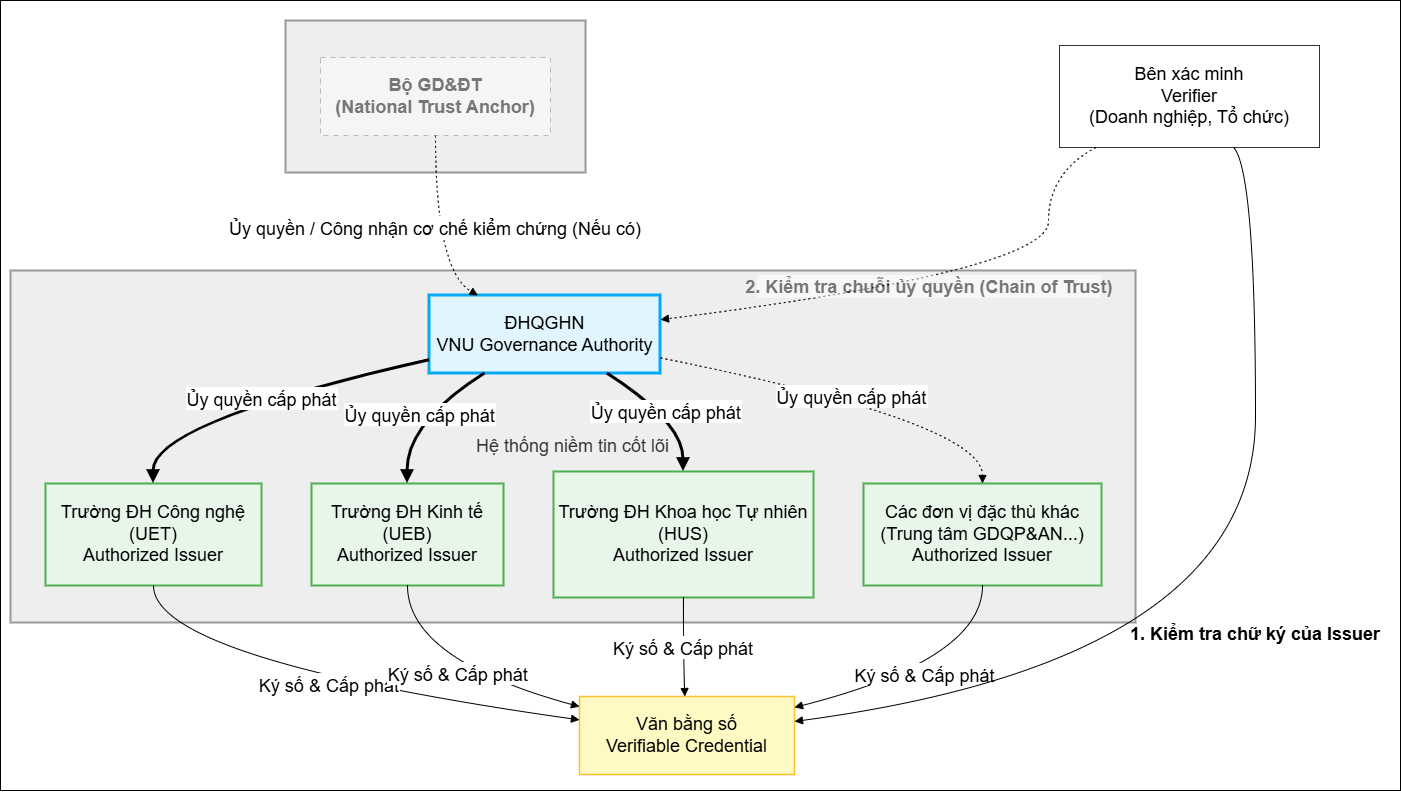
\includegraphics[width=0.78\textwidth]{images/trust-propagation-model.png}
    \caption{Mô hình lan truyền niềm tin phân cấp trong hệ thống văn bằng số}
    \label{fig:v2-trust-propagation}
\end{figure}

Thành phần hiện thực hoá hai tầng trên là \emph{sổ đăng ký tin cậy} (trust registry), nơi lưu và công bố trạng thái của các bên phát hành: định danh, trạng thái, phạm vi được phép, thời hạn và quan hệ uỷ quyền. Trust over IP đã công bố Trust Registry Query Protocol 2.0 vào tháng 4/2026 \cite{ToIP_TRQP2026}, định nghĩa truy vấn về thẩm quyền và truy vấn về công nhận giữa các sổ, nhưng hoãn truy vấn về \emph{uỷ quyền nhiều cấp} sang phiên bản sau. Từ đó một khung quản trị cần năm đặc tính: tra cứu độc lập; thay đổi có hiệu lực ngay trong lần xác minh tiếp theo; phạm vi thẩm quyền tường minh chứ không nhị phân; dấu vết kiểm toán không xoá được kể cả bởi cơ quan quản trị; và tách khỏi lớp xác minh. Weigl và cộng sự nhấn mạnh thêm yêu cầu trạng thái quản trị phải ở dạng máy đọc được \cite{Weigl2025}.

\section{Khảo sát các hệ thống tiêu biểu}
\label{sec:khao-sat}

\textbf{Blockcerts} \cite{Blockcerts2016} biểu diễn chứng thực bằng JSON-LD, ký bằng khoá của bên phát hành và neo giá trị băm lên blockchain công khai. Hệ thống chứng minh từ rất sớm rằng xác minh độc lập là khả thi, nhưng không có sổ đăng ký tin cậy: tổ chức nào cũng sinh khoá và phát hành được. Khoảng trống này đã bị khai thác. Baldi và cộng sự chỉ ra một tấn công mạo danh: quy trình xác minh đối chiếu danh tính bên phát hành với một hồ sơ \emph{không được xác thực} do chính bên phát hành công bố, nên kẻ tấn công dựng được hồ sơ giả cùng chứng thực giả không phân biệt nổi với chứng thực thật \cite{Baldi2019}. Bảy năm sau, cùng nhóm báo cáo một tấn công giả mạo trên Block.co, một hệ thống thương mại, và quy nguyên nhân về việc thiếu một cơ quan có thẩm quyền ràng buộc danh tính pháp lý của tổ chức với danh tính số của bên phát hành \cite{Zonneveld2026}. Cả hai hệ thống bị tấn công đều có chữ ký hợp lệ và giá trị băm neo đúng cách. Thêm cơ chế mật mã không lấp được khoảng trống này.

\textbf{EDC và EBSI} của Liên minh Châu Âu \cite{EDC_ELM, EBSI_TrustModel} giải quyết đủ ba tầng. Các tổ chức kiểm định được tin cậy công nhận bên phát hành theo lĩnh vực và địa bàn, và bản thân sự công nhận cũng là một chứng thực; lược đồ chứng thực được đăng ký trong một sổ riêng. Hai nguyên tắc của EBSI được khoá luận kế thừa: sổ cái ghi nhận quyết định về niềm tin chứ không tạo ra chúng, và mỗi bên xác minh tự chọn gốc niềm tin. Hệ thống gắn với khung pháp lý eIDAS \cite{eIDAS2014}, được sửa đổi năm 2024 để lập Ví Định danh số Châu Âu \cite{eIDAS2_2024}. Đổi lại, toàn bộ hệ sinh thái phụ thuộc vào hạ tầng và cơ chế quản trị của Liên minh.

\textbf{Open Badges 3.0} \cite{OpenBadges2024} biểu diễn huy hiệu dưới dạng VC, giải quyết tốt tầng kỹ thuật và phù hợp với chứng nhận vi mô. Giá trị huy hiệu phụ thuộc vào uy tín xã hội của bên phát hành; không có khung quản trị thống nhất. Điều này hợp với mục đích của chuẩn nhưng không đáp ứng văn bằng chính quy.

\textbf{Trust over IP} \cite{ToIP_Stack2022} là kiến trúc tham chiếu bốn lớp kỹ thuật, với một chồng quản trị song song áp dụng ở mọi lớp \cite{ToIP_GovMetamodel2022}. Cách nhìn quản trị như một chiều xuyên suốt chính xác hơn coi nó là một lớp riêng. Hạn chế là dừng ở mức tham chiếu, không có mô hình triển khai cho giáo dục.

\textbf{EduCTX} \cite{Turkanovic2018} xác định rõ bài toán liên thông định danh giữa nhiều trường và biểu diễn tín chỉ dưới dạng token, nhưng không xử lý thẩm quyền cấp phát. Báo cáo của Trung tâm Nghiên cứu Chung thuộc Uỷ ban Châu Âu cũng cho rằng rào cản chính của blockchain trong giáo dục nằm ở quản trị và chuẩn hoá chứ không ở công nghệ \cite{Grech2017}.

\textbf{Các khung niềm tin trong nghiên cứu học thuật.} Ngoài các hệ thống đã triển khai, một nhóm công trình học thuật đề xuất trực tiếp cơ chế thiết lập niềm tin. Saramago và cộng sự biểu diễn văn bằng thành một tập chứng thực bất biến tổ chức theo cấu trúc cây với dấu thời gian liên kết, nhằm tạo minh bạch về quy trình của bên phát hành \cite{Saramago2021}; hướng này gần với hạ tầng minh bạch chứng thư và rất mạnh về tính toàn vẹn, nhưng ghi nhận chứ không thi hành quy tắc thẩm quyền. Eer, Diaz và Kohlweiss đề xuất sổ đăng ký tin cậy theo hướng từ dưới lên dựa trên uy tín, có cơ chế khuyến khích tham gia trung thực \cite{Eer2022}. De Salve và cộng sự đề xuất một khung niềm tin nhiều lớp dựa trên quan hệ tin cậy giữa các tác nhân, cài đặt bằng hợp đồng Solidity trên cả mạng riêng lẫn mạng công khai \cite{DeSalve2023}; đây là công trình gần nhất với khoá luận về phương pháp kiểm chứng. Weigl và cộng sự nhấn mạnh rằng trạng thái quản trị phải máy đọc được để ví tự đưa ra quyết định tin cậy \cite{Weigl2025}. Điểm chung của nhóm này là đi theo hướng \emph{uy tín phân tán} hoặc \emph{minh bạch}, phù hợp khi không có cơ quan quản trị được công nhận. Giáo dục đại học là trường hợp ngược lại: luôn có một cơ quan có thẩm quyền theo luật, nên một mô hình uỷ quyền thể chế có cấu trúc khớp với thực tiễn hơn.

\textbf{Bối cảnh Việt Nam.} Nền tảng blockchain quốc gia NDAChain ra mắt năm 2025 theo mô hình cấp phép, với tập nút xác thực được lựa chọn và giám sát, kèm một giải pháp định danh phi tập trung \cite{NDAChain2025}. Khung kiến trúc tổng thể quốc gia số công bố cuối năm 2025 xác định blockchain quốc gia là hạ tầng dùng chung. Hệ thống định danh điện tử công dân đã có độ phủ rộng, và theo Thông tư 10/2026/TT-BGDĐT \cite{TT10_2026}, tra cứu văn bằng trên nền tảng này có thể thay bản sao từ sổ gốc. Ở phía giáo dục, HEMIS quản lý dữ liệu vĩ mô của ngành và hệ thống văn bằng quốc gia cung cấp dịch vụ tra cứu. Các khối hạ tầng đã có, nhưng chúng đều trả lời câu hỏi ``bản ghi có tồn tại không''; lớp trả lời câu hỏi ``đơn vị này có thẩm quyền cấp loại văn bằng này không'' thì chưa được định hình. Vì vậy khung quản trị được thiết kế độc lập với nền tảng neo cụ thể, để có thể chuyển sang NDAChain mà không thiết kế lại.

\begin{table}[H]
\centering
\caption{Tổng hợp khảo sát theo ba tầng niềm tin}
\label{tab:v2-survey}
\renewcommand{\arraystretch}{1.25}
\small
\begin{tabular}{|p{2.2cm}|p{2.6cm}|p{3.4cm}|p{3.4cm}|p{1.6cm}|}
\hline
\textbf{Hệ thống} & \textbf{Kỹ thuật} & \textbf{Thể chế} & \textbf{Quản trị} & \textbf{Chủ thể giữ dữ liệu} \\ \hline
Blockcerts & Đầy đủ & Không có; đã bị khai thác \cite{Baldi2019} & Thu hồi qua danh sách bên phát hành tự giữ & Có \\ \hline
EDC/EBSI & Đầy đủ & Đầy đủ, qua tổ chức kiểm định & Đầy đủ nhưng tập trung vào hạ tầng Liên minh & Hạn chế \\ \hline
Open Badges 3.0 & Đầy đủ & Yếu, dựa vào uy tín xã hội & Không có khung thống nhất & Có \\ \hline
Trust over IP & Mức tham chiếu & Mô tả khái niệm & Mô tả đầy đủ nhất, không có triển khai & Theo thiết kế \\ \hline
EduCTX & Đầy đủ cho tín chỉ & Không phải trọng tâm & Không có cơ chế thu hồi thẩm quyền & Có \\ \hline
Mô hình đề xuất & Đầy đủ, có bước đối chiếu nội dung & Chuỗi thẩm quyền thành mã thi hành, có phạm vi và thời hạn & Công khai trên chuỗi, dấu vết không xoá được & Có \\ \hline
\end{tabular}
\end{table}


\section{Khoảng trống nghiên cứu}
\label{sec:khoang-trong}

Liệt kê khoảng trống thành một danh sách ngang hàng sẽ không cho biết một nghiên cứu đơn lẻ xử lý được tới đâu: khoảng trống ở tầng chuẩn hoá cần cả cộng đồng đồng thuận, còn khoảng trống ở tầng kiến trúc giải quyết được trong một hệ thống. Bảng \ref{tab:v2-gap} phân loại thành sáu tầng kèm phạm vi xử lý của khoá luận.

\begin{table}[H]
\centering
\caption{Phân loại khoảng trống nghiên cứu và phạm vi xử lý của khoá luận}
\label{tab:v2-gap}
\renewcommand{\arraystretch}{1.25}
\small
\begin{tabular}{|c|p{2.2cm}|p{5.6cm}|p{4.6cm}|}
\hline
\textbf{Mã} & \textbf{Tầng} & \textbf{Khoảng trống} & \textbf{Khoá luận} \\ \hline
G1 & Chuẩn hoá & Chuẩn truy vấn sổ đăng ký hoãn phần uỷ quyền nhiều cấp \cite{ToIP_TRQP2026}; chuẩn trạng thái không biểu diễn thẩm quyền & Góp một cách biểu diễn cụ thể chạy được \\ \hline
G2 & Kiến trúc & Sổ đăng ký là cơ sở dữ liệu của một tổ chức, chỉ di chuyển sự phụ thuộc \cite{SSI_Survey2025} & Xử lý trực tiếp: sổ đăng ký là trạng thái hợp đồng \\ \hline
G3 & Biểu diễn thẩm quyền & Thẩm quyền nhị phân, thiếu phạm vi, thời hạn, số cấp & Xử lý trực tiếp: mặt nạ bit, thời hạn, uỷ quyền hai cấp \\ \hline
G4 & Ngữ nghĩa xác minh & Không phân biệt loại thất bại; không đối chiếu nội dung với băm đã neo & Xử lý trực tiếp: bảy bước báo cáo riêng \\ \hline
G5 & Phương pháp đánh giá & Chỉ 2/47 công trình có nghiên cứu người dùng \cite{Ambati2026} & Không xử lý, cùng chung giới hạn \\ \hline
G6 & Bối cảnh & Pháp lý và hạ tầng đã có, thiếu lớp quản trị thẩm quyền cho giáo dục & Xử lý một phần, trong một trường hợp nghiên cứu \\ \hline
\end{tabular}
\end{table}


Ba tầng G2, G3 và G4 thuộc phạm vi kiến trúc nên được xử lý trực tiếp. Với G2, hướng của EBSI \emph{di chuyển} sự phụ thuộc từ nơi cấp lên tổ chức vận hành sổ đăng ký chứ không loại bỏ nó \cite{SSI_Survey2025}; khoá luận đặt sổ đăng ký thành trạng thái của hợp đồng trên chuỗi. Hướng này có công trình đi trước theo lối uy tín phân tán \cite{Eer2022, DeSalve2023}; khoá luận đi theo lối uỷ quyền thể chế có cấu trúc, phù hợp khi có cơ quan quản trị được công nhận, điều luôn đúng trong giáo dục đại học. Với G3, ba chiều thông tin bị thiếu trong biểu diễn nhị phân là phạm vi, thời hạn và số cấp uỷ quyền. Với G4, khi một chứng thực bị từ chối, bên xác minh cần biết đó là nội dung bị sửa, chứng thực bị thu hồi hay bên phát hành mất thẩm quyền, vì mỗi trường hợp cần một cách xử lý khác nhau.

G5 là khoảng trống mà khoá luận \emph{cũng mắc phải}. Ambati và cộng sự ghi nhận chỉ 2 trong 47 công trình được phân tích có nghiên cứu người dùng \cite{Ambati2026}; nghiên cứu hiếm hoi của Zaeem và cộng sự cho thấy người dùng thấy khó hiểu ở bước khởi tạo và lo mất khoá \cite{Zaeem2021}. Khoá luận cũng chỉ kiểm chứng bằng kiểm thử và đo đạc, nên kết luận của nó là về tính khả thi kỹ thuật chứ không về mức độ tiếp nhận. Với G1, khoá luận chỉ đóng góp một cách biểu diễn cụ thể cho phần chuẩn còn hoãn; với G6, khoá luận xử lý một phần trong phạm vi một trường hợp nghiên cứu.
